\documentclass[compress]{beamer}
\usepackage{irbookslide}
\usepackage{irilmenau2}
\usepackage{tikz}
\usepackage{url}
\usepackage{ifxetex}
%\RequireXeTeX
\usepackage{fontspec} % zahteva paket euenc
\usepackage{xunicode}
\usepackage{xltxtra}
\usepackage{polyglossia}
\usepackage{minted}
\usepackage[noend]{algorithmic}
\renewcommand{\algorithmicrequire}{\textbf{Input:}}
\renewcommand{\algorithmicensure}{\textbf{Output:}}
\usepackage{xcolor,colortbl}
\usepackage{textcomp}
\usepackage{unicode-math}
%\usepackage{hyphenat}
%\setdefaultlanguage[script=Latin]{serbian}

\title{Sortiranje i selekcija}
\author{\textcopyright \ \ Goodrich, Tamassia, Goldwasser}
\institute{Katedra za informatiku, Fakultet tehničkih nauka, Univerzitet u
Novom Sadu}
\date{2014.}
\subject{Predavanja sa ASP}

\begin{document}

\frame{\titlepage}

\begin{frame}[fragile]
  \frametitle{Sortiranje}
  \begin{itemize}
    \item \myred{sortiranje}: izmena redosleda elemenata u kolekciji tako da budu poređani od najmanjeg ka najvećem 
    \item videli smo da red sa prioritetom može da posluži za sortiranje
    \begin{itemize}
      \item \textbf{selection sort} je $O(n^2)$
      \item \textbf{insertion sort} je $O(n^2)$ 
      \item \textbf{heap sort} je $O(n\log n)$
    \end{itemize}
  \end{itemize}
\end{frame}

\section[Merge sort]{Merge sort}

\begin{frame}[fragile]
  \frametitle{Merge sort}
  \begin{itemize}
    \item \myred{merge sort} je primer \textbf{divide-and-conquer} šablona 
    \begin{itemize}
      \item \textbf{divide}: podeli $S$ na dva disjunktna podskupa $S_1$ i $S_2$
      \item \textbf{recur}: reši potproblem za $S_1$ i $S_2$ 
      \item \textbf{conquer}: kombinuj rešenja za $S_1$ i $S_2$ u rešenje za $S$
    \end{itemize}
    \item bazni slučaj za rekurziju je skup veličine 0 ili 1 
  \end{itemize}
\end{frame}

\begin{frame}[fragile]
  \frametitle{Merge sort}
  \begin{itemize}
    \item merge sort je $O(n\log n)$, kao i heap sort
    \item za razliku od heap sorta 
    \begin{itemize}
      \item ne koristi pomoćnu strukturu podataka (RSP)
      \item pristupa podacima sekvencijalno -- pogodno za sortiranje podataka na disku
    \end{itemize}
  \end{itemize}
\end{frame}

\begin{frame}[fragile]
  \frametitle{Merge sort algoritam}
  \begin{columns}
    \begin{column}[t]{6cm}
      \begin{itemize}
        \item sortira sekvencu $S$ dužine $n$ u tri koraka
        \item[1] \myred{divide}: podeli $S$ na $S_1$ i $S_2$, svaki dužine $~n/2$
        \item[2] \myred{recur}: rekurzivno sortiraj $S_1$ i $S_2$
        \item[3] \myred{conquer}: spoj sortirane $S_1$ i $S_2$ u sortiranu sekvencu
      \end{itemize}    
    \end{column}
    \begin{column}[t]{6cm}
      \myred{mergeSort}($S$)
      \begin{algorithmic}
      \REQUIRE sekvenca $S$ sa $n$ elemenata
      \ENSURE sortirana sekvenca $S$
      \IF{len($S$) $>1$}
        \STATE $(S_1, S_2) \leftarrow$ partition($S, n/2$)
        \STATE mergeSort($S_1$)
        \STATE mergeSort($S_2$)
        \STATE $S \leftarrow$ merge($S_1$, $S_2$)
      \ENDIF
      \end{algorithmic}    
    \end{column}
  \end{columns}
\end{frame}

\begin{frame}[fragile,shrink]
  \frametitle{Spajanje sortiranih sekvenci}
  \myred{merge}($A, B$)
  \begin{algorithmic}
    \REQUIRE sekvenca $A$ i $B$ sa $n/2$ elemenata svaka
    \ENSURE sortirana sekvenca $A\cup B$
    \STATE $S \leftarrow$ prazna sekvenca
    \WHILE{$\neg A.isEmpty() \land \neg B.isEmpty()$}
      \IF{$A.first().element() < B.first().element()$}
        \STATE $S.addLast(A.remove(A.first()))$
      \ELSE
        \STATE $S.addLast(B.remove(B.first()))$
      \ENDIF
    \ENDWHILE
    \WHILE{$\neg A.isEmpty()$}
      \STATE $S.addLast(A.remove(A.first()))$
    \ENDWHILE
    \WHILE{$\neg B.isEmpty()$}
      \STATE $S.addLast(B.remove(B.first()))$
    \ENDWHILE
  \end{algorithmic}    
\end{frame}

\begin{frame}[fragile,shrink]
  \frametitle{Spajanje sortiranih sekvenci}
\begin{minted}[linenos=false]{python}
def merge(s1, s2, s):
  i = j = 0
  while i + j < len(s):
    if j == len(s2) or (i < len(s1) and s1[i] < s2[j]):
      s[i+j] = s1[i]
      i += 1
    else:
      s[i+j] = s2[i]
      j += 1
\end{minted}
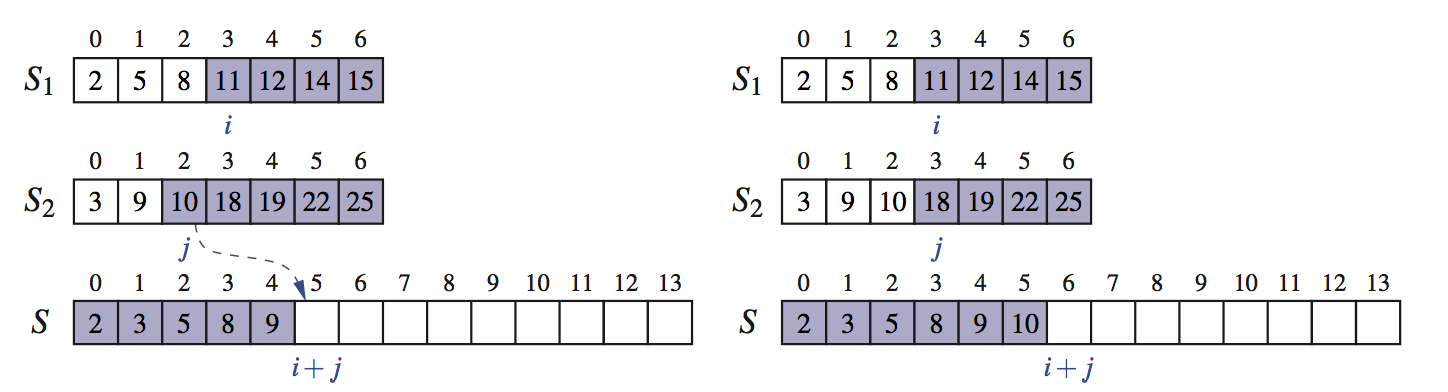
\includegraphics[width=11cm]{asp-12-pic01.png}
\end{frame}

\begin{frame}[fragile,shrink]
  \frametitle{Merge sort u Pythonu}
\begin{minted}[linenos=false]{python}
def merge_sort(s):
  n = len(s)
  if n < 2:
    return  # already sorted
  # divide
  mid = n//2
  s1 = s[0:mid]
  s2 = s[mid:n]
  # recur
  merge_sort(s1)
  merge_sort(s2)
  # conquer
  merge(s1, s2, s)
\end{minted}
\end{frame}

\begin{frame}[fragile]
  \frametitle{Stablo sortiranja}
  \begin{itemize}
    \item izvršavanje merge sorta može se prikazati binarnim stablom
    \item čvor stabla predstavlja jedan rekurzivni poziv i čuva
    \begin{itemize}
      \item nesortiranu sekvencu pre podele
      \item sortiranu sekvencu nakon završetka
    \end{itemize}
    \item koren je početni poziv funkcije
    \item listovi su pozivi sa podsekvence dužine 0 ili 1
  \end{itemize}
  \begin{center}
    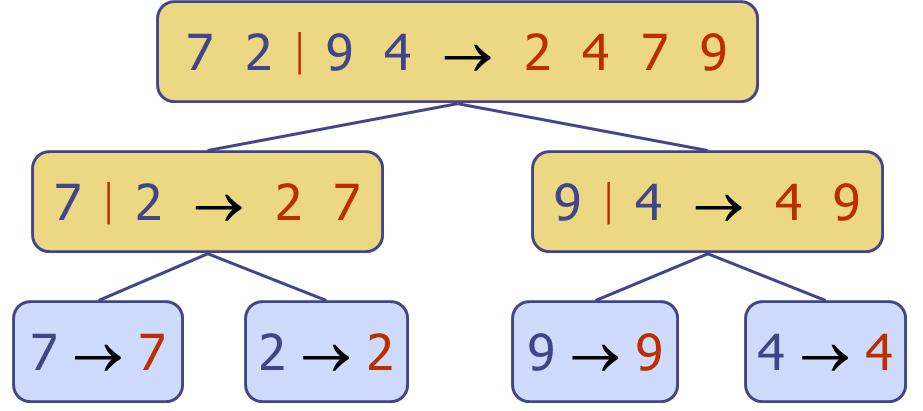
\includegraphics[width=7cm]{asp-12-pic02.png}
  \end{center}
\end{frame}
  
\begin{frame}[fragile]
  \frametitle{Primer sortiranja}
  \begin{itemize}
    \only<1>{\item podela}
    \only<2>{\item rekurzija, podela}
    \only<3>{\item rekurzija, podela}
    \only<4>{\item rekurzija, bazni slučaj}
    \only<5>{\item rekurzija, bazni slučaj}
    \only<6>{\item spajanje}
    \only<7>{\item rekurzija, \ldots, bazni slučaj, spajanje}
    \only<8>{\item spajanje}
    \only<9>{\item rekurzija, \ldots, spajanje, spajanje}
    \only<10>{\item spajanje}
  \end{itemize}
  \begin{center}
    \includegraphics<1>[width=11cm]{asp-12-pic03.png}
    \includegraphics<2>[width=11cm]{asp-12-pic04.png}
    \includegraphics<3>[width=11cm]{asp-12-pic05.png}
    \includegraphics<4>[width=11cm]{asp-12-pic06.png}
    \includegraphics<5>[width=11cm]{asp-12-pic07.png}
    \includegraphics<6>[width=11cm]{asp-12-pic08.png}
    \includegraphics<7>[width=11cm]{asp-12-pic09.png}
    \includegraphics<8>[width=11cm]{asp-12-pic10.png}
    \includegraphics<9>[width=11cm]{asp-12-pic11.png}
    \includegraphics<10>[width=11cm]{asp-12-pic12.png}
  \end{center}
\end{frame}

\begin{frame}[fragile]
  \frametitle{Merge sort: performanse}
  \begin{itemize}
    \item visina $h$ stabla za merge sort je $O(\log n)$
    \begin{itemize}
      \item delimo sekvencu na pola za svaku rekurziju
    \end{itemize}
    \item ukupan broj operacija na nivou $i$ je $O(n)$
    \begin{itemize}
      \item delimo i spajamo $2^i$ sekvenci dužine $n/2^i$
      \item pravimo $2^{i+1}$ rekurzivnih poziva
    \end{itemize}
    \item ukupno vreme izvršavanja je $O(n\log n)$
  \end{itemize}
  \begin{center}
    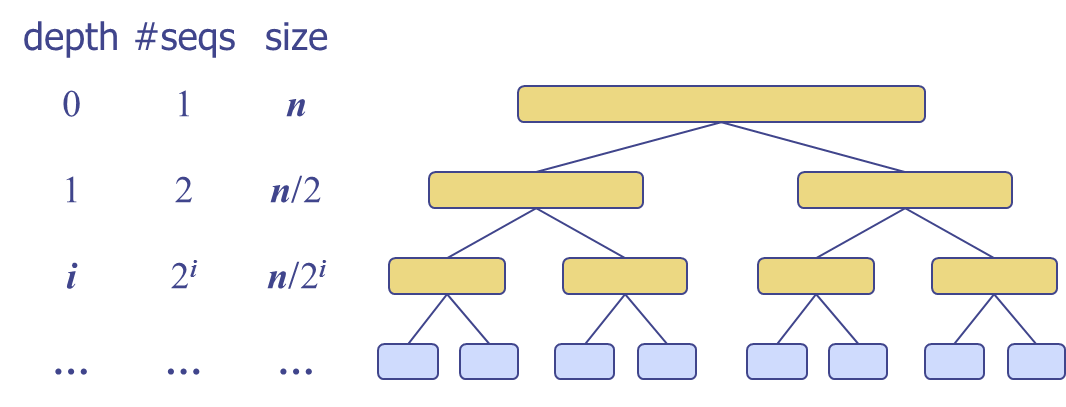
\includegraphics[width=9cm]{asp-12-pic13.png}
  \end{center}
\end{frame}

\begin{frame}[fragile]
  \frametitle{Algoritmi za sortiranje (za sada)}
  \begin{tabular}{l|c|p{6cm}}
  \textbf{algoritam} & \textbf{vreme} & \textbf{napomene} \\ \hline\hline
   &  & $\rhd$ spor \\ 
  selection & $O(n^2)$ & $\rhd$ in-place \\ 
   &  & $\rhd$ za male sekvence (< 1K) \\ \hline
   &  & $\rhd$ spor \\ 
  insertion & $O(n^2)$ & $\rhd$ in-place \\ 
   &  & $\rhd$ za male sekvence (< 1K) \\ \hline
   &  & $\rhd$ brz \\
  heap & $O(n\log n)$ & $\rhd$ in-place \\
   &  & $\rhd$ za velike sekvence (1K-1M) \\ \hline
   &  & $\rhd$ brz \\
  merge & $O(n\log n)$ & $\rhd$ sekvencijalan \\
   &  & $\rhd$ za ogromne sekvence (> 1M) \\ \hline
  \end{tabular}
\end{frame}

\begin{frame}[fragile,shrink=25]
  \frametitle{Merge sort: nerekurzivna varijanta $_1$}
\begin{minted}[linenos=false]{python}
def merge_sort(S):
  """Sort the elements of Python list S using the merge-sort algorithm."""
  n = len(S)
  logn = math.ceil(math.log(n,2))
  src, dest = S, [None] * n             # make temporary storage for dest
  for i in (2**k for k in range(logn)): # pass i creates all runs of length 2i
    for j in range(0, n, 2*i):          # each pass merges two length i runs
      merge(src, dest, j, i)
    src, dest = dest, src               # reverse roles of lists
  if S is not src:
    S[0:n] = src[0:n]                   # additional copy to get results to S
\end{minted}
\end{frame}

\begin{frame}[fragile,shrink=25]
  \frametitle{Merge sort: nerekurzivna varijanta $_2$}
\begin{minted}[linenos=false]{python}
def merge(src, result, start, inc):
  """Merge src[start:start+inc] and src[start+inc:start+2*inc]."""
  end1 = start+inc                   # boundary for run 1
  end2 = min(start+2*inc, len(src))  # boundary for run 2
  x, y, z = start, start+inc, start  # index into run 1, run 2, result
  while x < end1 and y < end2:
    if src[x] < src[y]:
      result[z] = src[x]
      x += 1
    else:
      result[z] = src[y]
      y += 1
    z += 1                           # increment z to reflect new result
  if x < end1:
    result[z:end2] = src[x:end1]     # copy remainder of run 1 to output
  elif y < end2:
    result[z:end2] = src[y:end2]     # copy remainder of run 2 to output
\end{minted}
\end{frame}

\section[Quick sort]{Quick sort}

\begin{frame}[fragile]
  \frametitle{Quick sort}
  \begin{columns}
    \begin{column}[t]{6cm}
      \begin{itemize}
        \item \myred{quick sort} je \textit{randomized} podeli-pa-vladaj algoritam
        \item[1] \myred{divide}: izaberi slučajan element $x$ (\myred{pivot}) i podeli $S$ na
        \begin{itemize}
          \item $L$: elementi manji od $x$
          \item $E$: elementi jednaki $x$
          \item $G$: elementi veći od $x$
        \end{itemize}    
        \item[2] \myred{recur}: sortiraj $L$ i $G$
        \item[3] \myred{conquer}: spoj sortirane $L$, $E$ i $G$
      \end{itemize}    
    \end{column}
    \begin{column}[t]{6cm}
      \begin{center}
        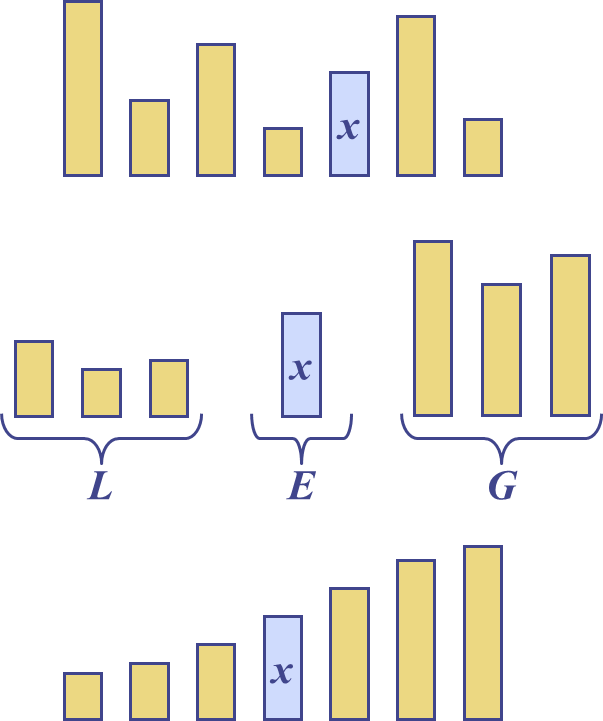
\includegraphics[width=5cm]{asp-12-pic14.png}
      \end{center}
    \end{column}
  \end{columns}
\end{frame}

\begin{frame}[fragile,shrink]
  \frametitle{Particija ulaza}
  \myred{partition}($S, p$)
  \begin{algorithmic}
    \REQUIRE sekvenca $S$ i pozicija pivota $p$
    \ENSURE sekvence $L$, $E$, $G$
    \STATE $L,E,G \leftarrow$ prazne sekvence
    \STATE $x \leftarrow S$.remove($p$) 
    \WHILE{$\neg S.isEmpty()$}
      \STATE $y \leftarrow S$.remove($S$.first())
      \IF{$y < x$}
        \STATE $L$.addLast($y$)
      \ELSIF{$y = x$}
        \STATE $E$.addLast($y$)
      \ELSE 
        \STATE $G$.addLast($y$)
      \ENDIF
    \ENDWHILE
    \RETURN $L,E,G$
  \end{algorithmic}
  \hfill particija je $O(n)$    
\end{frame}

\begin{frame}[fragile]
  \frametitle{Stablo sortiranja}
  \begin{itemize}
    \item izvršavanje quick sorta može se prikazati binarnim stablom
    \item čvor stabla predstavlja jedan rekurzivni poziv i čuva
    \begin{itemize}
      \item nesortiranu sekvencu pre podele oko pivota
      \item sortiranu sekvencu nakon završetka
    \end{itemize}
    \item koren je početni poziv funkcije
    \item listovi su pozivi sa podsekvence dužine 0 ili 1
  \end{itemize}
  \begin{center}
    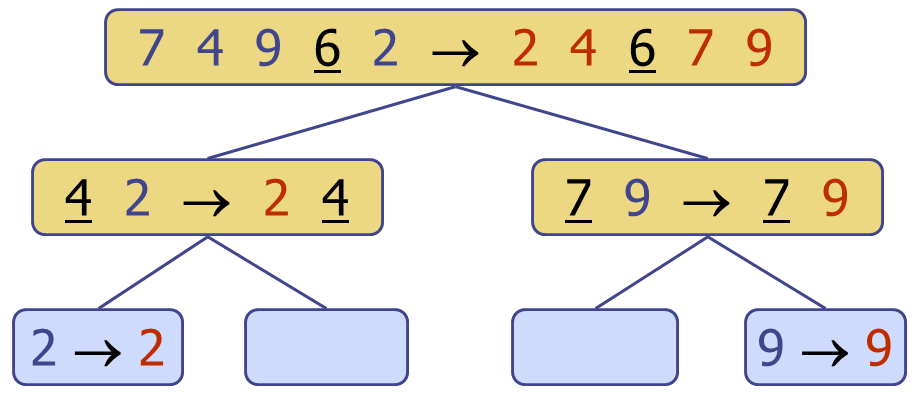
\includegraphics[width=7cm]{asp-12-pic15.png}
  \end{center}
\end{frame}

\begin{frame}[fragile]
  \frametitle{Primer sortiranja}
  \begin{itemize}
    \only<1>{\item izbor pivota}
    \only<2>{\item particija, rekurzija, izbor pivota}
    \only<3>{\item particija, rekurzija, bazni slučaj}
    \only<4>{\item rekurzija, \ldots, bazni slučaj, spajanje}
    \only<5>{\item rekurzija, izbor pivota}
    \only<6>{\item particija, \ldots, rekurzija, bazni slučaj}
    \only<7>{\item spajanje, spajanje}
  \end{itemize}
  \begin{center}
    \includegraphics<1>[width=11cm]{asp-12-pic16.png}
    \includegraphics<2>[width=11cm]{asp-12-pic17.png}
    \includegraphics<3>[width=11cm]{asp-12-pic18.png}
    \includegraphics<4>[width=11cm]{asp-12-pic19.png}
    \includegraphics<5>[width=11cm]{asp-12-pic20.png}
    \includegraphics<6>[width=11cm]{asp-12-pic21.png}
    \includegraphics<7>[width=11cm]{asp-12-pic22.png}
  \end{center}
\end{frame}

\begin{frame}[fragile]
  \frametitle{Performanse u najgorem slučaju}
  \begin{itemize}
    \item najgori slučaj: kada je pivot najveći ili najmanji element
    \item jedan od $L$ ili $G$ ima dužinu 0 a drugi dužinu $n-1$
    \item vreme izvršavanja je tada proporcionalno sumi
    $$ n + (n-1) + \ldots + 2 + 1$$
    \item $\Rightarrow$ najgori slučaj je $O(n^2)$
  \end{itemize}
  \begin{center}
    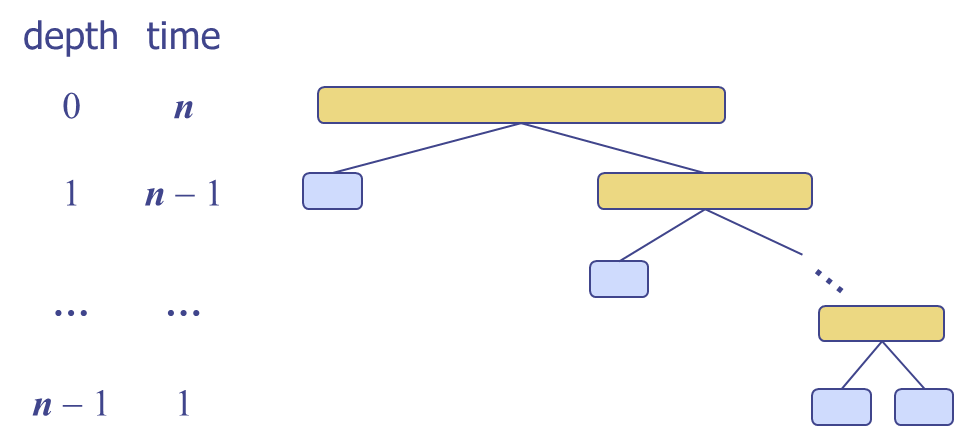
\includegraphics[width=8cm]{asp-12-pic23.png}
  \end{center}
\end{frame}

\begin{frame}[fragile]
  \frametitle{Očekivane performanse}
  \begin{itemize}
    \item posmatrajmo rekurzivni poziv za sekvencu dužine $s$
    \begin{itemize}
      \item \myred{dobar izbor}: dužine $L$ i $G$ su obe manje od $s\cdot 3/4$
      \item \myred{loš izbor}: $L$ ili $G$ ima dužinu veću od $s\cdot 3/4$
    \end{itemize}
  \end{itemize}
  \begin{center}
    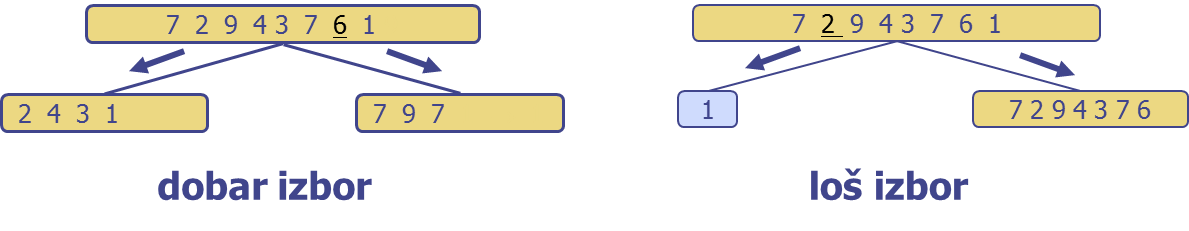
\includegraphics[width=10cm]{asp-12-pic24.png}
  \end{center}
  \begin{itemize}
    \item slučajan izbor pivota je dobar sa verovatnoćom $1/2$
    \begin{itemize}
      \item $1/2$ mogućih pivota su dobar izbor
    \end{itemize}
  \end{itemize}
  \begin{center}
    
\includegraphics[width=6cm]{asp-12-pic25.png}
  \end{center}
\end{frame}

\begin{frame}[fragile]
  \frametitle{Očekivane performanse}
  \begin{itemize}
    \item iz verovatnoće: očekivani broj bacanja novčića da bismo dobili $k$ glava je $2k$
    \item za čvor dubine $i$ očekujemo
    \begin{itemize}
      \item $i/2$ predaka su dobri izbori
      \item veličina ulazne sekvence za tekući poziv je najviše $n\cdot (3/4)^{i/2}$
    \end{itemize}
  \end{itemize}
  \begin{columns}
    \begin{column}[t]{5cm}
      {\scriptsize
      \begin{itemize}
        \item za čvor dubine $2\log_{4/3}n$ očekivana veličina ulaza je 1
        \item očekivana visina stabla je $O(\log n)$
        \item broj operacija za čvorove iste dubine je $O(n)$
        \item $\Rightarrow$ ukupno očekivano vreme quick sorta je $O(n\log n)$ 
      \end{itemize}
      }
    \end{column}
    \begin{column}[t]{7cm}
      \begin{center}
        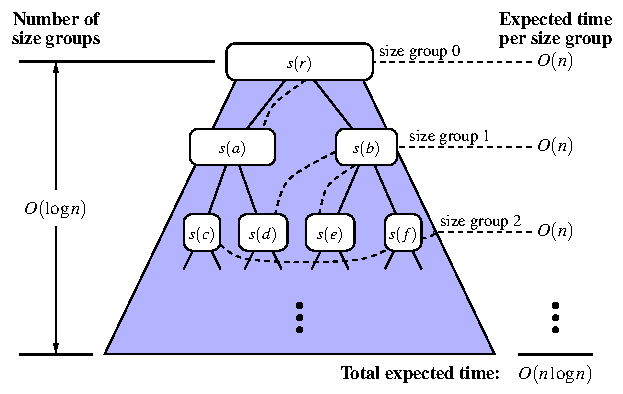
\includegraphics[width=7cm]{asp-12-pic26.pdf}
      \end{center}
    \end{column}
  \end{columns}
\end{frame}

\begin{frame}[fragile]
  \frametitle{In-place particija}
  \begin{itemize}
    \item koristimo indekse $j$ i $k$ da podelimo $S$ na dva dela: $L$ i $E\cup G$
  \end{itemize}
  \begin{center}
    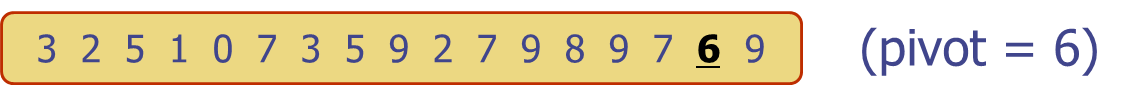
\includegraphics[width=10cm]{asp-12-pic26.png}
  \end{center}
  \begin{itemize}
    \item ponavljaj dok se $j$ i $k$ ne mimoiđu ($k<j$)
    \begin{itemize}
      \item pomeraj $j$ u desno dok ne naiđemo na element $\geq x$ 
      \item pomeraj $k$ u levo dok ne naiđemo na element $< x$
      \item zameni elemente na pozicijama $i$ i $k$ 
    \end{itemize}
  \end{itemize}
  \begin{center}
    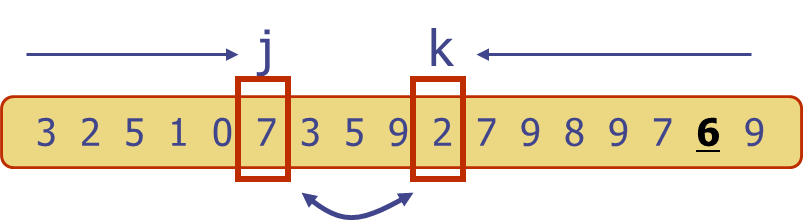
\includegraphics[width=6cm]{asp-12-pic27.png}
  \end{center}
\end{frame}

\begin{frame}[fragile,shrink=25]
  \frametitle{In-place quick sort}
\begin{minted}[linenos=false]{python}
def inplace_quick_sort(S, a, b):
  """Sort the list from S[a] to S[b] inclusive using quick-sort."""
  if a >= b: return                           # range is trivially sorted
  pivot = S[b]                                # last element of range is pivot
  left = a                                    # will scan rightward
  right = b-1                                 # will scan leftward
  while left <= right:
    # scan until reaching value equal or larger than pivot (or right marker)
    while left <= right and S[left] < pivot:
      left += 1
    # scan until reaching value equal or smaller than pivot (or left marker)
    while left <= right and pivot < S[right]:
      right -= 1
    if left <= right:                         # scans did not strictly cross
      S[left], S[right] = S[right], S[left]   # swap values
      left, right = left + 1, right - 1       # shrink range

  # put pivot into its final place (currently marked by left index)
  S[left], S[b] = S[b], S[left]
  # make recursive calls
  inplace_quick_sort(S, a, left - 1)
  inplace_quick_sort(S, left + 1, b)
\end{minted}
\end{frame}

\begin{frame}[fragile]
  \frametitle{Algoritmi za sortiranje (za sada)}
  \begin{tabular}{l|c|p{6cm}}
  \textbf{algoritam} & \textbf{vreme} & \textbf{napomene} \\ \hline\hline
  selection & $O(n^2)$ & $\rhd$ in-place \\ 
   &  & $\rhd$ spor (dobar za male ulaze) \\ \hline
  insertion & $O(n^2)$ & $\rhd$ in-place \\ 
   &  & $\rhd$ spor (dobar za male ulaze) \\ \hline
  heap & $O(n\log n)$ & $\rhd$ in-place \\
   &  & $\rhd$ brz (dobar za velike ulaze) \\ \hline
  merge & $O(n\log n)$ & $\rhd$ sekvencijalan \\
   &  & $\rhd$ brz (dobar za ogromne ulaze) \\ \hline
  quick & $O(n\log n)$ & $\rhd$ in-place, randomized \\
   & {\tiny očekivano} & $\rhd$ najbrži (dobar za velike ulaze) \\ \hline
  \end{tabular}
\end{frame}

\section[Granice brzine]{Granice brzine}

\begin{frame}[fragile]
  \frametitle{Sortiranje zasnovano na poređenju}
  \begin{itemize}
    \item mnogi algoritmi se zasnivaju na poređenju elemenata
    \begin{itemize}
      \item porede se parovi elemenata 
      \item bubble, selection, insertion, heap, merge, quick\ldots
    \end{itemize}
    \item postoji li donja granica za vreme potrebno ovakvim algoritmima koji sortiraju $x_1, x_2, \ldots, x_n$?
  \end{itemize}
  \begin{center}
    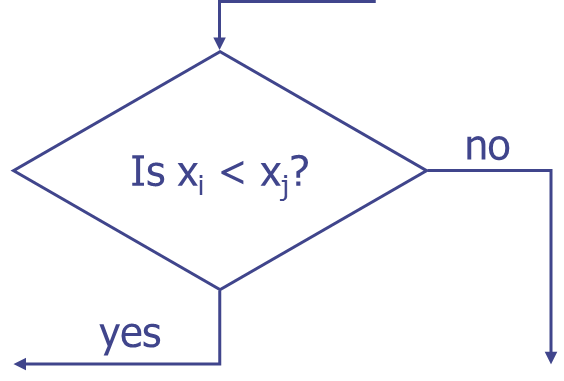
\includegraphics[width=5cm]{asp-12-pic28.png}
  \end{center}
\end{frame}

\begin{frame}[fragile]
  \frametitle{Brojanje operacija poređenja}
  \begin{itemize}
    \item svako pokretanje algoritma odgovara jednoj putanji koren$\rightarrow$list u \myred{stablu odlučivanja}
  \end{itemize}
  \begin{center}
    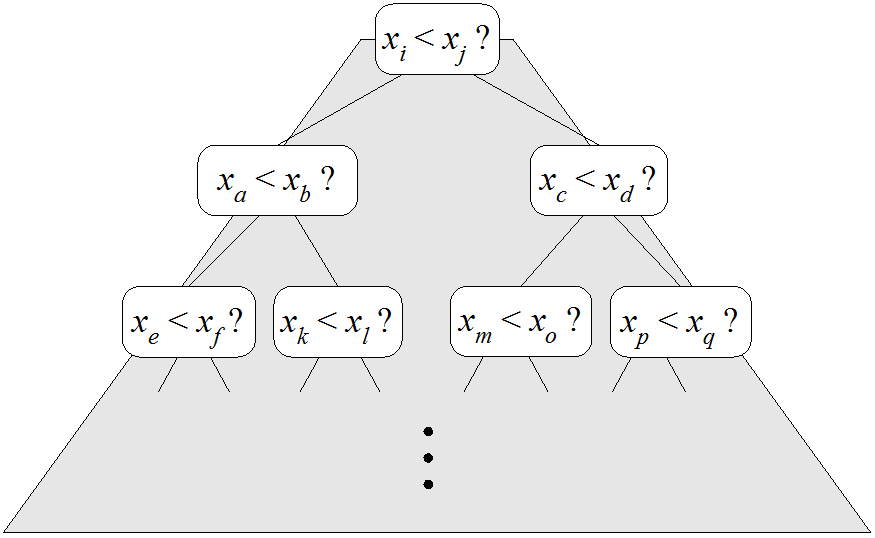
\includegraphics[width=8cm]{asp-12-pic29.png}
  \end{center}
\end{frame}

\begin{frame}[fragile]
  \frametitle{Stablo odlučivanja}
  \begin{itemize}
    \item visina stabla odlučivanja je donja granica za vreme sortiranja
    \item svaka permutacija ulaza vodi do posebnog lista
    \item stablo ima $n!$ listova $\Rightarrow$ visina stabla je barem $O(n!)$
  \end{itemize}
  \begin{center}
    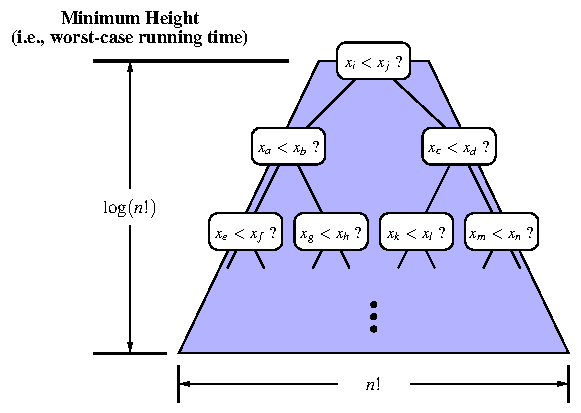
\includegraphics[width=8cm]{asp-12-pic30.pdf}
  \end{center}
\end{frame}

\begin{frame}[fragile]
  \frametitle{Granica brzine}
  \begin{itemize}
    \item svaki algoritam koji se zasniva na poređenju je barem $O(n!)$
    \item prema tome, vreme izvšavanja svakog algoritma je najmanje
    $$\log n! \geq \log \left(\frac{n}{2}\right)^{\frac{n}{2}} = \frac{n}{2}\log\frac{n}{2}$$
    \item tj. svaki ovakav algoritam je $\Omega(n\log n)$
  \end{itemize}
\end{frame}

\section[Bucket sort]{Bucket sort}

\end{document}
